\section{Filter Parameters}
Given the project specifications, it is possible to draw the \textbf{Data Flow Diagram} as shown in \autoref{lab1:fig:iir-dfd}.
\begin{figure}[htbp]
	\center
	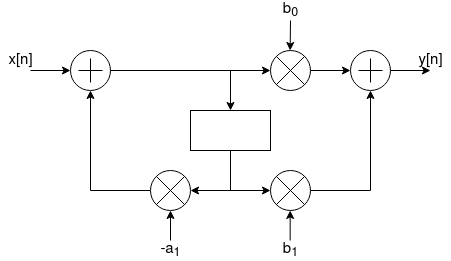
\includegraphics[width=0.65\textwidth]{chapter1/images/iir-dfd.png}
	\caption{Target filter data flow diagram}
	\label{lab1:fig:iir-dfd}
\end{figure}

Given the basic structure, it is necessary to determine the values of the $a$ and $b$ parameters. After feeding the specifications in the provided Matlab script \texttt{myiir\_design.m}, the results are:
\begin{align}
    a &= [-21] \\
    b &= [53,\ 53]
\end{align}


As defined in the project specifications, the filter is going to be implemented in hardware and will use an 8 bit \textbf{fixed point} representation: this simplifies the structure of the filter, but limits its precision.\\
To properly verify the functionality of the filter, it is necessary to have a reference model that also works with 8 bit fixed point numbers. In addition, this allows for an insightful comparison of the filter's behavior when it is working in floating point (in Matlab) versus fixed point, which is going to be implemented in C.

Truly fixed point operation is modeled in a C program where coefficients and data are stored using the standard \texttt{int} data type. A scale factor equal to $2^{n_b-1}$ is implied and input values to this program are rescaled within the same Matlab script where they are generated in order to match the full scale range of an $n_b$-bits two's complement representation.  Sums and multiplications are 

